\section*{Diskuze}


Trubice C měla jen velmi malou oblast laminárního proudění, při výšce vodního sloupce 4,5~cm již bylo proudění nestabilní a hladina velmi kolísala. Pro velmi malé tlaky byl naopak průtok téměř neměřitelný. V oblasti laminárního proudění jsme tedy provedli jen dvě měření a při fitování závislosti \eqref{eq:fit} jsme měli k dispozici stejný počet bodů jako fitovaných parametrů. Navíc první ze dvou měření ($h =$ 1,6~cm) mohlo být zatíženo hrubou chybou, voda vytékala částečně po vnějších stěnách trubice a je možné, že se do odměrného válce nepodařila odchytit všechna. Graf \ref{graf:k_na_Re} navíc napovídá, že druhé z těchto dvou měření ($Re =$1088, $k =$ 0.024) již proběhlo při turbulentním proudění, přestože hladina v manometrické trubici ještě nekolísala. Vzhledem k těmto skutečnostem odchylku parametrů mírně nadhodnotíme a určíme s ohledem na odchylky obou bodů (viz obrázek \ref{graf:chybaC}).


\begin{figure}[htbp] 
\centering
% GNUPLOT: LaTeX picture with Postscript
\begingroup
  \makeatletter
  \providecommand\color[2][]{%
    \GenericError{(gnuplot) \space\space\space\@spaces}{%
      Package color not loaded in conjunction with
      terminal option `colourtext'%
    }{See the gnuplot documentation for explanation.%
    }{Either use 'blacktext' in gnuplot or load the package
      color.sty in LaTeX.}%
    \renewcommand\color[2][]{}%
  }%
  \providecommand\includegraphics[2][]{%
    \GenericError{(gnuplot) \space\space\space\@spaces}{%
      Package graphicx or graphics not loaded%
    }{See the gnuplot documentation for explanation.%
    }{The gnuplot epslatex terminal needs graphicx.sty or graphics.sty.}%
    \renewcommand\includegraphics[2][]{}%
  }%
  \providecommand\rotatebox[2]{#2}%
  \@ifundefined{ifGPcolor}{%
    \newif\ifGPcolor
    \GPcolortrue
  }{}%
  \@ifundefined{ifGPblacktext}{%
    \newif\ifGPblacktext
    \GPblacktextfalse
  }{}%
  % define a \g@addto@macro without @ in the name:
  \let\gplgaddtomacro\g@addto@macro
  % define empty templates for all commands taking text:
  \gdef\gplbacktext{}%
  \gdef\gplfronttext{}%
  \makeatother
  \ifGPblacktext
    % no textcolor at all
    \def\colorrgb#1{}%
    \def\colorgray#1{}%
  \else
    % gray or color?
    \ifGPcolor
      \def\colorrgb#1{\color[rgb]{#1}}%
      \def\colorgray#1{\color[gray]{#1}}%
      \expandafter\def\csname LTw\endcsname{\color{white}}%
      \expandafter\def\csname LTb\endcsname{\color{black}}%
      \expandafter\def\csname LTa\endcsname{\color{black}}%
      \expandafter\def\csname LT0\endcsname{\color[rgb]{1,0,0}}%
      \expandafter\def\csname LT1\endcsname{\color[rgb]{0,1,0}}%
      \expandafter\def\csname LT2\endcsname{\color[rgb]{0,0,1}}%
      \expandafter\def\csname LT3\endcsname{\color[rgb]{1,0,1}}%
      \expandafter\def\csname LT4\endcsname{\color[rgb]{0,1,1}}%
      \expandafter\def\csname LT5\endcsname{\color[rgb]{1,1,0}}%
      \expandafter\def\csname LT6\endcsname{\color[rgb]{0,0,0}}%
      \expandafter\def\csname LT7\endcsname{\color[rgb]{1,0.3,0}}%
      \expandafter\def\csname LT8\endcsname{\color[rgb]{0.5,0.5,0.5}}%
    \else
      % gray
      \def\colorrgb#1{\color{black}}%
      \def\colorgray#1{\color[gray]{#1}}%
      \expandafter\def\csname LTw\endcsname{\color{white}}%
      \expandafter\def\csname LTb\endcsname{\color{black}}%
      \expandafter\def\csname LTa\endcsname{\color{black}}%
      \expandafter\def\csname LT0\endcsname{\color{black}}%
      \expandafter\def\csname LT1\endcsname{\color{black}}%
      \expandafter\def\csname LT2\endcsname{\color{black}}%
      \expandafter\def\csname LT3\endcsname{\color{black}}%
      \expandafter\def\csname LT4\endcsname{\color{black}}%
      \expandafter\def\csname LT5\endcsname{\color{black}}%
      \expandafter\def\csname LT6\endcsname{\color{black}}%
      \expandafter\def\csname LT7\endcsname{\color{black}}%
      \expandafter\def\csname LT8\endcsname{\color{black}}%
    \fi
  \fi
  \setlength{\unitlength}{0.0500bp}%
  \begin{picture}(6802.00,4534.00)%
    \gplgaddtomacro\gplbacktext{%
      \csname LTb\endcsname%
      \put(682,704){\makebox(0,0)[r]{\strut{} 0}}%
      \csname LTb\endcsname%
      \put(682,1298){\makebox(0,0)[r]{\strut{} 1}}%
      \csname LTb\endcsname%
      \put(682,1892){\makebox(0,0)[r]{\strut{} 2}}%
      \csname LTb\endcsname%
      \put(682,2487){\makebox(0,0)[r]{\strut{} 3}}%
      \csname LTb\endcsname%
      \put(682,3081){\makebox(0,0)[r]{\strut{} 4}}%
      \csname LTb\endcsname%
      \put(682,3675){\makebox(0,0)[r]{\strut{} 5}}%
      \csname LTb\endcsname%
      \put(682,4269){\makebox(0,0)[r]{\strut{} 6}}%
      \csname LTb\endcsname%
      \put(814,484){\makebox(0,0){\strut{} 0}}%
      \csname LTb\endcsname%
      \put(1513,484){\makebox(0,0){\strut{} 50}}%
      \csname LTb\endcsname%
      \put(2212,484){\makebox(0,0){\strut{} 100}}%
      \csname LTb\endcsname%
      \put(2911,484){\makebox(0,0){\strut{} 150}}%
      \csname LTb\endcsname%
      \put(3610,484){\makebox(0,0){\strut{} 200}}%
      \csname LTb\endcsname%
      \put(4308,484){\makebox(0,0){\strut{} 250}}%
      \csname LTb\endcsname%
      \put(5007,484){\makebox(0,0){\strut{} 300}}%
      \csname LTb\endcsname%
      \put(5706,484){\makebox(0,0){\strut{} 350}}%
      \csname LTb\endcsname%
      \put(6405,484){\makebox(0,0){\strut{} 400}}%
      \put(176,2486){\rotatebox{-270}{\makebox(0,0){\strut{}$Q_v [ml \cdot s^{-1}]$}}}%
      \put(3609,154){\makebox(0,0){\strut{}$p \text{[Pa]}$}}%
    }%
    \gplgaddtomacro\gplfronttext{%
    }%
    \gplbacktext
    \put(0,0){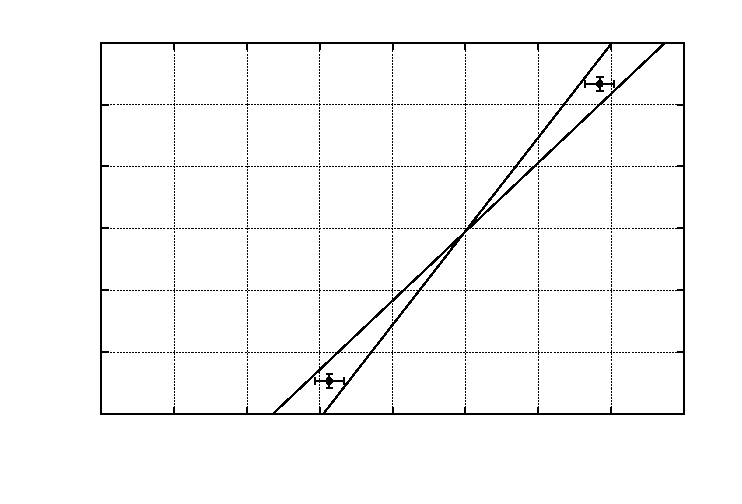
\includegraphics{grafdisk}}%
    \gplfronttext
  \end{picture}%
\endgroup

\caption{ První dva změřené body v oblasti laminárního proudění pro trubici C. Dvě přímky \mbox{$Q_v=(a+\sigma a)\cdot p+(b-\sigma b)$}, \mbox{$Q_v=(a-\sigma a)\cdot p+(b+\sigma b)$} ilustrují odhadnutou odchylku parametrů $a$ a $b$.}
\label{graf:chybaC}
\end{figure}

Opravené poloměry se s těmi naměřenými přiliš neshodují, naměřené jsou vždy vyšší. Jedním možným vysvětlením je neodhalená systematická chyba při měření posuvným měřítkem. Poloměr jsme měřili tím způsobem, že jsme dovnitř trubice strčili pacičky měřítka a roztáhli je na celý průměr trubice. Posuvné měřítko bylo plastové, takže je možné, že jsme působili přiliš velkou silou, pacičky se deformovali a naměřili jsme vyšší hodnotu.

Závislost $k(Re)$ vyšla podle očekávání. Trubice A měla nejmenší poloměr, při všech měřeních v ní voda proudila laminárně a závislost přesně odpovídá teoretické. U trubice C proběhly všechny měření kromě prvních dvou při turbulentním proudění a závislost téměř přesně odpovídá teoretické pro turbulentní proudění. V trubici B bylo nejdříve laminární proudění a přibližně při $Re=$1300 začalo být nestabilní. Pro $Re>$2000 bylo již proudění trvale turbulentní. Skutečně hodnoty $k$ nejdříve odpovídají křivce pro laminární proudění a poté se začínají blížit té pro turbulentní.